% !TEX root = ../thesis.tex
%
\setcounter{chapter}{2}
\chapter{Fostering Com\-pu\-ta\-tion\-al Think\-ing Skills with Vi\-su\-al Pro\-gram\-ming Lan\-guages}\label{chap:exploration}

\cleanchapterquote{Education means making creators... You have to make inventors, innovators, not conformists.}{Jean Piaget}{Conversations with Jean Piaget, 1980}

The previous chapter presented an overview of the existing research related to \ac{CT} and \acp{TUI}. This chapter carries on with the primary thesis investigation on the effects of tangible interaction on the development of \ac{CT} skills and focuses on existing tools used in education and their effects on promoting such skills.

\section{Introduction}
As discussed in the introduction, today's society is increasingly surrounded by technology, and it is unmistakably clear how much people rely on software in every part of their lives. That being the case, people will always strive to play a more active role in their life, thus programming is becoming an essential skill to master for the general public, resulting in an overall heightened interest in coding. Take for instance the Hour of Code~\cite{HOC}, a successful global initiative organised by Code.org (a non-profit organisation founded in 2013 and supported, among others, by Mark Zuckerberg and Bill Gates) involving millions of students of different ages starting with 4-year old, aiming at introducing coding skills to a broader and mixed audience.

Programming is no longer just a job skill but has turned into a literacy, enabling people to acquire a new way of thinking and looking at the world, fostering the so-called \ac{CT} skills, i.e.\ abilities like problem-solving, abstraction, and pattern recognition to name but a few. They empower people to break complex problems down into small chunks and express them to a computer~\cite{Vee:2013wc}. \ac{CT} shares many of its concepts, practices, and perspectives with other subject areas taught in schools, such as science, mathematics, arts, and engineering, making a strong case for its promotion in disciplines outside of \ac{CS} and right from kindergarten~\cite{Namukasa:2015wj} as a new form of literacy~\cite{Vee:2013wc}.

Due to this sudden global interest in promoting \ac{CT} skills to many broad and diverse audiences, several tools and methods have been designed with the aim of supporting the introduction of programming concepts in more effective and less daunting ways than the past. A popular theory of learning that can come to the aid on this matter is Piaget's constructivism~\cite{Piaget:1969vq}, which argues that people produce knowledge and form new meanings based upon their experiences and social interactions. Exploiting them to teach those concepts underpinning \ac{CT} might represent an effective and engaging way of supporting the learning of such skills.

\acp{TUI}~\cite{Ishii:1997gy} are an interaction paradigm that was devised to foster collaborative learning and exploit humans' natural dexterity for physical objects manipulation to provide an easy to use interface that can be used even by inexperienced people. They exploit the physical world to offer a concrete representation of the abstract concepts learners usually struggle with and thus could be a valid way of fostering \ac{CT} skills~\cite{McNerney:2004jc,Horn:2009be}.

To recap, from this context discerns the main Research Question addressed by this thesis: \textit{``Do the collaborative and cognitive naturalness of physical objects manipulation at the basis of \acp{TUI} aid the understanding of core algorithmic principles and \replaced[comment={D1}]{thus improve}{thus improving} \ac{CT} skills?''}.

In the past few years the echo of the discussion around the importance of teaching programming and \ac{CT} in school~\cite{Anonymous:2011kk} resounded in the introduction of coding as part of their national curriculum by many European nations (such as England, Finland, and Estonia) and many other countries (e.g., Russia, South Africa, New Zealand, and Australia~\cite{Balanskat:aDdZD1gb}) either already have or plan to introduce \ac{CS} as part of their K-12 curriculum~\cite{Grover:2013gj}.

Currently, many educational events and lectures are introducing \ac{CT} to newcomers and learners all around the world. Teachers are supported by a wide variety of multi-purpose technological tools mostly designed to target their scenarios and needs. The majority of them are digital tools using a \ac{VPL} (e.g., Scratch) that allows users to program simple tasks by manipulating graphical elements on the screen. Many studies have been carried out investigating these tools in terms of their effects on programming ability or attitude, though not much discussion has arisen about their effects on collaborative learning of \ac{CT} in real-world educational scenarios.

Tools and methods applied within these educational domains tend to nurture collaboration amongst learners rather than individual activities to facilitate peer discussion and feedback, exploiting learning through direct experiences as suggested by constructivist theories.

The Research Question derived from this context and addressed in this chapter is then: \textit{``Can existing \ac{VPL}-based tools support the collaborative learning of \ac{CT} skills?''}.

This chapter presents an evaluation of an existing \ac{VPL}-based technological tool --- i.e.\ OzoBlockly~\cite{OZOB} --- and currently used in introductory programming sessions to teach \ac{CT} skills concerning its support to collaborative learning of \ac{CT}. The study took place in a real-world environment, analysing an actual introductory programming sessions as they were carried out in a real educational institution by practitioners, without any intervention of researchers. It established a snapshot of today's main tools supporting \ac{CT} and how new ones might improve upon their shortcomings and exploit their strengths.

\section{Related Works}\label{sec:rw3}
\acp{VPL} are a particular breed of programming languages that allow users to program by manipulating graphical elements on the screen rather than textual as in traditional programming environments~\cite{jost2014graphical}. Recently they have been adopted in many educational scenarios, thanks to their ease of use and efficacy in lowering the entry barriers of professional programming systems.

\acp{VPL} fall into two broad categories, namely Block-based, which falls di\-rect\-ly from the im\-per\-a\-tive par\-a\-digm on tra\-di\-tion\-al pro\-gram\-ming lan\-guages, or Flow-based, which discerns from traditional functional programming languages~\cite{mason2017block}. Even though there have not been many empirical studies evaluating the benefits of one against the other, in recent years many new Block-based \ac{VPL} have been developed and successfully employed in introducing programming to children and fostering their \ac{CT} skills in different scenarios and events.

The main principle guiding the \acp{VPL}-based tools' development was the ``low floor, high ceiling'' approach --- i.e.\ the tool enables any beginner to cross the threshold to create working programs easily (low floor), but they are also powerful enough to satisfy the needs of more advanced users (high ceiling). Other effective tool features for promoting \ac{CT} skills are represented by
\begin{enumerate*}[label=(\arabic*)]
  \item providing stepping stones with managed skills and challenges, to get them from the ``floor'' to the ``ceiling'' (scaffold);
  \item enable transfer between different application contexts;
  \item support equity;
  \item be systemic and sustainable~\cite{Repenning:2010cz}.
\end{enumerate*}

\acp{VPL}-based tools like Scratch~\cite{Resnick:2009bd}, Alice~\cite{Herbert:2012}, Kodu~\cite{Fowler:2012}, Blockly~\cite{trower2015blockly}, and App Inventor~\cite{gray2012teaching}, closely follow these 5 principles \replaced[comment={D7}]{to varying degrees}{on various degrees}: they are relatively easy to use and allow novices to focus on design and creating while avoiding the issues of the traditional murky and complicated programming syntax.

They engage in \ac{CT} using a three-stage ``Use-Modify-Create'' pattern~\cite{Lee:2011tm}, scaffolding increasingly deep interaction to foster the development of \ac{CT} skills; users start using existing artefacts and gain confidence through a series of iterative modifications and refinements, as well as fostering appropriation of what started as someone else's and became one's own.

These tools, however, need to support --- and, in turn, be supported --- by curricular activities such as educational robotics and game design, typically serving as a trigger for the iterative exploration of \ac{CT} while motivating and engaging school children.

These activities should support what have been proposed to be the four pedagogical phases of learning to think computationally~\cite{Namukasa:2015wj}:
\begin{enumerate}
  \item unplugged (off-screen) activities, to inspire students and enhance subject knowledge, making abstract concepts both tangible and visible, and improving upon their problem-solving skills;
  \item making activities that include playing or making things, encouraging students to cohesively combine multiple ideas~\cite{WilkersonJerde:2014ve};
  \item tinkering~\cite{Bers:2014fk}, support learning of \ac{CT} concepts and exploring in a creative way, providing a rich context for developing and representing understanding through the experience and building process~\cite{Papert:1980uh};
  \item remixing (or ``hacking'') involves critically looking at an existing code, as well as practising modifying it to suit new purposes; analyzing code, making connections and creating new applications from existing code requires sophisticated reasoning and problem-solving skills.
\end{enumerate}

Lastly, it is worth pointing out that the effectiveness of existing \ac{VPL}-based tools seems pretty unsettled with respect to the many facets of \ac{CT}: for instance, a 2008 study~\cite{Maloney:2008jt} involving 80 urban youth aged 8--18 reported learning of several \ac{CT} elements through the use of Scratch in an after-school setting; nonetheless, the tool does not provide a mean of encapsulating functionalities into procedures and functions, somehow failing to tap into the abstraction skills. There is undoubtedly a need for new tools that foster \ac{CT} skills specifically targeted to K-12 education, following the principles just described and guided by the most recent research on how children approach problem-solving~\cite{Chen:2007hc,Pane:2001jo}.

\section{Evaluation}
This section presents the goals and hypotheses and describes the ex\-per\-i\-ments car\-ried out to e\-val\-u\-ate ex\-ist\-ing tech\-no\-log\-i\-cal tools sup\-port\-ing \ac{CT}, and is or\-gan\-ised fol\-low\-ing the guide\-lines of the A\-mer\-i\-can Psychological Association~\cite{Wohlin:2000:ESE:330775}.

\subsection{Goals}
The goal of the study is to compare collaboratively working learners with individual working ones for the purpose of evaluating \ac{CT} skills development in the context of using a \ac{VPL}-based technological tool, namely OzoBlockly, in a real-world introductory robot programming session. The purpose is to test whether \ac{VPL}-based tools are suitable to cultivate \ac{CT} skills in real-world collaborative learning scenarios.

\subsection{Research Question}
Nowadays programming is not just a job skill, but it is rather an ability that enables people to acquire a new way of thinking and to look at the world, fostering mental skills such as problem-solving, abstraction, and pattern recognition to name but a few, the so-called \ac{CT} skills. They empower people to break complex problems down into small chunks and express them to a computer~\cite{Vee:2013wc}.

Currently, technological tools used to introduce \ac{CT} to newcomers in educational scenarios are mostly graphical tools using a \ac{VPL}. Over the past few years, many advantages of such interaction paradigm have been studied and discussed in relation to programming ability and effects on the entry barriers, but its effects on collaborative learning of \ac{CT} skills have been somewhat disregarded.

The Research Question derived from this context and addressed by this study is then: \textit{``Can existing \ac{VPL}-based tools support the collaborative learning of \ac{CT} skills?''}.

\subsection{Experiment Design}
A standard between-subjects design with one factor and two treatments were used~\cite{Wohlin:2000:ESE:330775}. The treatments correspond to 
\begin{enumerate*}[label={(\roman*)}]
  \item programming sessions with learners working individually (control group), and
  \item programming sessions with learners working collaboratively in groups (experiment group).
\end{enumerate*}

\subsection{Participants}
The participants of the experiments were 88 Key Stage 3 (aged between 11 and 14) students coming from 5 classes of different schools in the London \replaced[comment={D8}]{Borough of Hillingdon area, all with comparable socio-economic level}{area}. The control group was composed by 25 individually working students from 2 of the 5 different schools (15 from one, 10 from another), while the experimental group consisted of 26 groups of students coming from the remaining 3 (15, 30, 18 from each), clustered in 15 groups of 2 students and 11 of 3 because of space and resources constraints.

Some students had some minimal programming experience --- mostly with Scratch --- but the vast majority had never programmed before. No prerequisite knowledge was required to participate, and none of the participants had prior knowledge of the setup of the experiment.

\subsection{Settings and Experiment Tasks}
The context of the experiment was robot programming, an activity often chosen as an engaging introduction to \ac{CT} in educational events and sessions, as discussed in chapter~\ref{chap:background}. The \ac{VPL}-based tool selected for the evaluation was OzoBlockly~\cite{OZOB}, an online programming environment based on Google's Blockly~\cite{BLOCKLY}, allowing users to develop small programs by manipulating graphical elements on the screen. It can be used to control the movements and behaviour of Ozobots, small wheeled robots capable of moving autonomously and emitting lights. The programming environment doesn't require knowledge of any specific programming language and provides several types of instructions such as navigation, light effects, timing, and loops, all grouped by function, as depicted in figure~\ref{fig:ozoblockly}. Once a user is happy with the outcome, the program can be sent to the robot through an optical sensor and executed by pressing a button on the side of the robot.

\begin{figure}[ht!]
  \centering
  \includegraphics[width=0.75\textwidth,trim={0 80 500 0},clip]{images/c3/OzoBlockly.png} 
  \caption{The OzoBlockly programming environment.}\label{fig:ozoblockly}
\end{figure}

The study took place in a laboratory inside the Department of Computer Science within the Brunel University London facilities.

Each group was provided with an Android tablet locked on the OzoBlockly Web page, a fully-charged Ozobot, and a set of small pins.

The experiment took place during an actual \ac{CT} introductory session, and the tasks consisted of a series of challenges of increasing difficulty to be completed by programming the Ozobot. The first required participants to make the robot do a simple turn and hit a pin at the end of the track. The second and third ones extended the first by requiring always an extra turn to hit the pin, making the track longer and more challenging. Finally, three pins were lined up in front of the robot at a similar distance to one another, requiring participants to dodge each one of them in sequence to complete the race.

Tasks were designed to require multiple trials from learners to be as accurate as possible, fostering the reuse of previous solutions without being too challenging for inexperienced users.

Students were presented with each challenge and asked to try and solve it by themselves, with facilitators assisting students when needed. There was no automatic verification of the results, as the purpose of the educational session was not to evaluate their programming skills, but rather to introduce them to \ac{CT} skills and engage them in controlling a robot. All the interactions and programs developed and sent to the robot were timed and recorded transparently, without interfering with the users' workflow.

\subsection{Procedure}
The experiment was carried out in one-hour long sessions, each involving a cohort coming from a single school, for a total of 5 different sessions.

Each session was chaired by one instructor, and no altering interventions were put in place by researchers, maintaining the actual schedule and tasks that were designed for the sessions. It started with a brief tutorial explaining the mechanics of the Ozobots, the OzoBlockly environment, and the process of sending programs to the robot.

Then participants were asked to try and develop a simple program making the robot move in a straight line, showing them how to do it first as an example.

After that, each challenge was introduced collaboratively and presented on a big screen by the facilitator. Participants were given 10 minutes to complete each task before introducing the next one, allowing them to try different strategies and discuss amongst teammates.

\subsection{Experiment Variables and Formalized Hypotheses}
The main independent variable of the experiment is group type and indicates whether a group was composed by more than one participant working together (denoted by ``C'') or by a single member working alone (denoted by ``I'').

As discussed in the previous chapter, measuring and defining exactly what \ac{CT} encompasses is still under lots of discussions within the scientific community, but many proposed definitions mention programs sequentialization and loops as two fundamental and easily measurable concepts underpinning it. In order to keep at the minimum the intervention on a real-world scenario for the experiment, the study focused on actual tasks prompted in an existing educational session, and the measures were designed to be the least intrusive as possible in order to obtain more truthful data. Also, time-based measures were disregarded, since the point of such introductory sessions is not the evaluation of participants' programming capability, but rather to support them in practising their \ac{CT} skills.

Thus, the main dependent variables selected for the experiment are the average length of sequential instruction issued together to the robot throughout an entire group session (shortened SEQ) --- which could be related to the understanding of sequences, a core concept of \ac{CT} --- and the average number of loops used in each program sent to the robot (shortened CYC) --- which could relate to the understanding of loops, another core \ac{CT} concept.

The research question was formalised into the following hypotheses:
\setcounter{hyp}{-1}\begin{hyp}[Null hypothesis]
  There are no differences in \ac{CT} skills development between learners working collaboratively and learners working individually when supported by a \ac{VPL}-based tool.
\end{hyp}
\begin{hyp}[Alternate hypothesis]
  There is a difference in \ac{CT} skills development between learners working collaboratively and learners working individually when supported by a \ac{VPL}-based tool, thus employing such tools in collaborative learning scenarios affects the development of \ac{CT} skills.
\end{hyp}

Table~\ref{tab:hypotheses} presents the experiment hypotheses formally in terms of the dependent variables. In the table, ``I'' refers to learners working individually (control group) and ``G'' refers to learners working collaboratively (experiment group).

\begin{table}[ht!]
  \caption{Formalized Hypotheses: SEQ is the average length of sequential instruction issued together to the robot throughout a group session, while CYC is the average number of loops used in each program sent to the robot within the same session; ``I'' refers to learners working individually (control group) and ``G'' refers to learners working collaboratively (experiment group).}\label{tab:hypotheses}
  \centering
  \begin{tabular}{cc}
    \toprule
    Null Hypothesis (\(H_0\)) & Alternate Hypothesis (\(H_1\)) \\
    \midrule
    \(SEQ_{I} = SEQ_{G}\) & \(SEQ_{I} \neq SEQ_{G}\) \\
    \(CYC_{I} = CYC_{G}\) & \(CYC_{I} \neq CYC_{G}\) \\
    \bottomrule
  \end{tabular}
\end{table}

\subsection{Summary}
\added[comment={MP3, MP8, D9, D11}]{To recap, table \ref{tab:ch3summary} presents a summary of the specific \ac{CT} dimensions as defined in~\cite{Brennan:2012} examined in the evaluation, along with the related assessment approach, as reported in the previous chapter.}

\begin{table}[ht!]
  \caption{Summary of the specific \ac{CT} dimensions~\cite{Brennan:2012} considered by the evaluation with the related assessment approach.}\label{tab:ch3summary}
  \centering
  \begin{tabular}{M{0.2\linewidth}m{0.5\linewidth}M{0.2\linewidth}}
    \toprule
    \textit{\ac{CT} Dimension} & \textit{Description} & \textit{Assessment} \\
    \midrule
    Concept: sequences & Ex\-press\-ing a par\-tic\-u\-lar ac\-tiv\-i\-ty or task as a se\-ries of in\-di\-vid\-u\-al steps or in\-struc\-tions that can be ex\-e\-cut\-ed by the com\-put\-er. & Project Analysis (SEQ) \\
    Concept: loops & Rec\-og\-niz\-ing rep\-e\-ti\-tions in a se\-quence of in\-struc\-tions and ex\-press\-ing it in a more suc\-cinct and ab\-stract way. & Project Analysis (CYC) \\
    \bottomrule
  \end{tabular}
\end{table}

\section{Results}
Fifty-one data points were obtained from the experiment, 25 for the control group (I), and 26 for the experimental group (G). The total number of valid programs issued to the robots was \numprint{4653}: \numprint{2423} from the control group, and \numprint{2230} from the experimental group.

\begin{figure}[ht!]
  \centering
  \input{images/c3/progs}
  \caption{Boxplot for the number of valid programs issued by each group.}\label{fig:programs}
\end{figure}

Figure~\ref{fig:programs} shows the boxplot for the number of programs issued to the robot by each experimental group. The average was \(96.92\) (standard deviation \(33.48\)) for learners working individually, and \(85.77\) (standard deviation \(38.05\)) for learners working collaboratively, thus \replaced[comment={D10}]{both groups issued a quite similar number of programs}{not a sensible difference in terms of the number of issued programs was recorded}. This was mostly expected, since tasks, setup, and available time was the same for all the participating groups. The slightly smaller average reported by the experimental group might be due to having a single control point (the tablet) and compromising between the perhaps different views of team members.

Moving on to measures related to the experimental hypotheses, the boxplot in figure~\ref{fig:avgs} shows the average number of sequential instructions issued to the robot across the different experimental groups (SEQ). The average was \(4.79\) (standard deviation \(1.35\)) for learners working individually, and \(4.21\) (standard deviation \(1.95\)) for learners working collaboratively, thus it would seem that working individually prompts the use of slightly more sequential blocks when performing the same tasks.

\begin{figure}[ht!]
  \centering
  % Created by tikzDevice version 0.12 on 2018-09-20 18:19:13
% !TEX encoding = UTF-8 Unicode
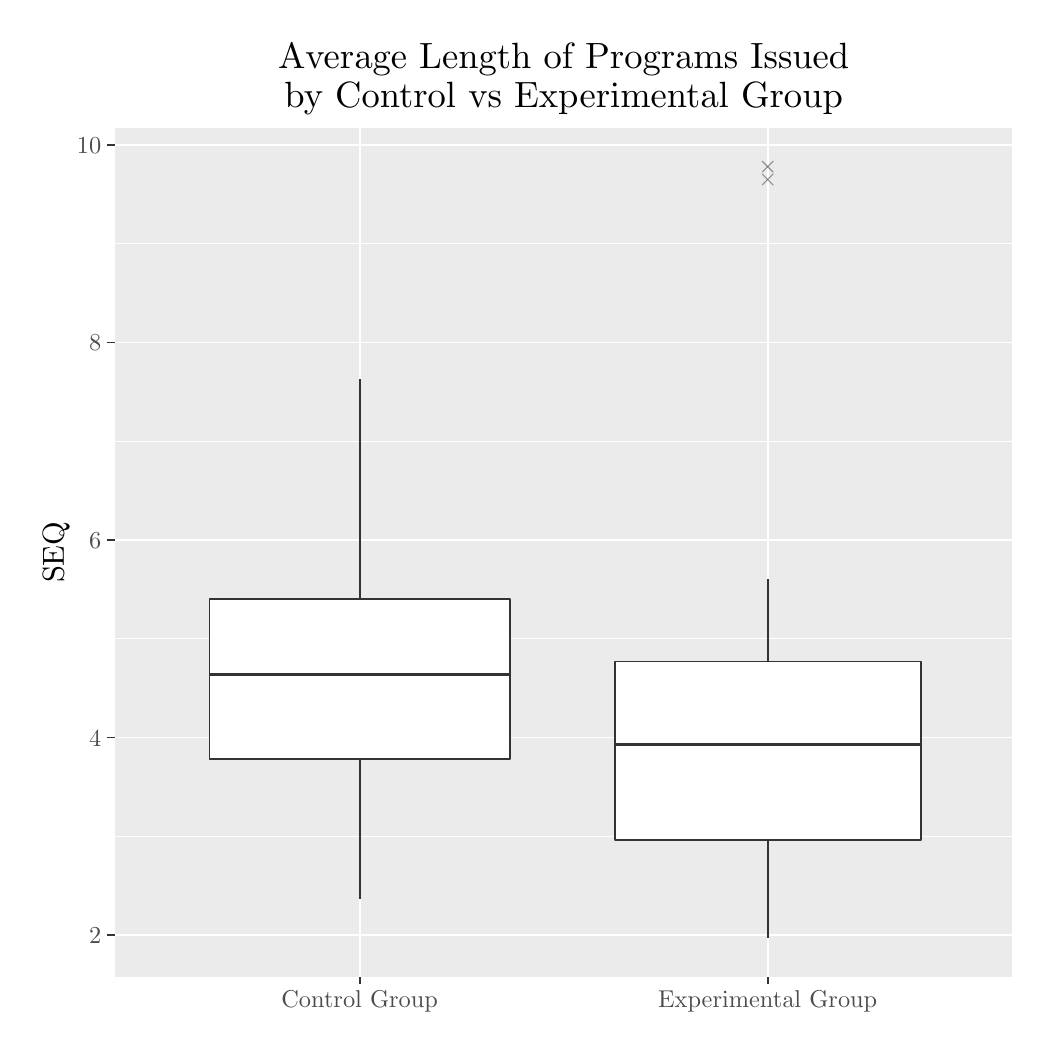
\begin{tikzpicture}[x=1pt,y=1pt]
\definecolor{fillColor}{RGB}{255,255,255}
\path[use as bounding box,fill=fillColor,fill opacity=0.00] (0,0) rectangle (361.35,361.35);
\begin{scope}
\path[clip] (  0.00,  0.00) rectangle (361.35,361.35);
\definecolor{drawColor}{RGB}{255,255,255}
\definecolor{fillColor}{RGB}{255,255,255}

\path[draw=drawColor,line width= 0.6pt,line join=round,line cap=round,fill=fillColor] (  0.00,  0.00) rectangle (361.35,361.35);
\end{scope}
\begin{scope}
\path[clip] ( 31.52, 18.45) rectangle (355.85,325.06);
\definecolor{fillColor}{gray}{0.92}

\path[fill=fillColor] ( 31.52, 18.45) rectangle (355.85,325.06);
\definecolor{drawColor}{RGB}{255,255,255}

\path[draw=drawColor,line width= 0.3pt,line join=round] ( 31.52, 69.12) --
	(355.85, 69.12);

\path[draw=drawColor,line width= 0.3pt,line join=round] ( 31.52,140.51) --
	(355.85,140.51);

\path[draw=drawColor,line width= 0.3pt,line join=round] ( 31.52,211.89) --
	(355.85,211.89);

\path[draw=drawColor,line width= 0.3pt,line join=round] ( 31.52,283.27) --
	(355.85,283.27);

\path[draw=drawColor,line width= 0.6pt,line join=round] ( 31.52, 33.43) --
	(355.85, 33.43);

\path[draw=drawColor,line width= 0.6pt,line join=round] ( 31.52,104.81) --
	(355.85,104.81);

\path[draw=drawColor,line width= 0.6pt,line join=round] ( 31.52,176.20) --
	(355.85,176.20);

\path[draw=drawColor,line width= 0.6pt,line join=round] ( 31.52,247.58) --
	(355.85,247.58);

\path[draw=drawColor,line width= 0.6pt,line join=round] ( 31.52,318.97) --
	(355.85,318.97);

\path[draw=drawColor,line width= 0.6pt,line join=round] (119.97, 18.45) --
	(119.97,325.06);

\path[draw=drawColor,line width= 0.6pt,line join=round] (267.40, 18.45) --
	(267.40,325.06);
\definecolor{drawColor}{RGB}{51,51,51}

\path[draw=drawColor,draw opacity=0.50,line width= 0.4pt,line join=round,line cap=round] (265.43,304.53) -- (269.36,308.46);

\path[draw=drawColor,draw opacity=0.50,line width= 0.4pt,line join=round,line cap=round] (265.43,308.46) -- (269.36,304.53);

\path[draw=drawColor,draw opacity=0.50,line width= 0.4pt,line join=round,line cap=round] (265.43,309.16) -- (269.36,313.08);

\path[draw=drawColor,draw opacity=0.50,line width= 0.4pt,line join=round,line cap=round] (265.43,313.08) -- (269.36,309.16);
\definecolor{drawColor}{gray}{0.20}

\path[draw=drawColor,line width= 0.6pt,line join=round] (267.40,132.27) -- (267.40,162.16);

\path[draw=drawColor,line width= 0.6pt,line join=round] (267.40, 67.74) -- (267.40, 32.39);
\definecolor{fillColor}{RGB}{255,255,255}

\path[draw=drawColor,line width= 0.6pt,line join=round,line cap=round,fill=fillColor] (212.11,132.27) --
	(212.11, 67.74) --
	(322.68, 67.74) --
	(322.68,132.27) --
	(212.11,132.27) --
	cycle;

\path[draw=drawColor,line width= 1.1pt,line join=round] (212.11,102.30) -- (322.68,102.30);

\path[draw=drawColor,line width= 0.6pt,line join=round] (119.97,154.78) -- (119.97,234.31);

\path[draw=drawColor,line width= 0.6pt,line join=round] (119.97, 96.97) -- (119.97, 46.41);

\path[draw=drawColor,line width= 0.6pt,line join=round,line cap=round,fill=fillColor] ( 65.76,154.78) --
	( 65.76, 96.97) --
	(174.18, 96.97) --
	(174.18,154.78) --
	( 65.76,154.78) --
	cycle;

\path[draw=drawColor,line width= 1.1pt,line join=round] ( 65.76,127.53) -- (174.18,127.53);
\end{scope}
\begin{scope}
\path[clip] (  0.00,  0.00) rectangle (361.35,361.35);
\definecolor{drawColor}{gray}{0.30}

\node[text=drawColor,anchor=base east,inner sep=0pt, outer sep=0pt, scale=  0.88] at ( 26.57, 30.40) {2};

\node[text=drawColor,anchor=base east,inner sep=0pt, outer sep=0pt, scale=  0.88] at ( 26.57,101.78) {4};

\node[text=drawColor,anchor=base east,inner sep=0pt, outer sep=0pt, scale=  0.88] at ( 26.57,173.17) {6};

\node[text=drawColor,anchor=base east,inner sep=0pt, outer sep=0pt, scale=  0.88] at ( 26.57,244.55) {8};

\node[text=drawColor,anchor=base east,inner sep=0pt, outer sep=0pt, scale=  0.88] at ( 26.57,315.94) {10};
\end{scope}
\begin{scope}
\path[clip] (  0.00,  0.00) rectangle (361.35,361.35);
\definecolor{drawColor}{gray}{0.20}

\path[draw=drawColor,line width= 0.6pt,line join=round] ( 28.77, 33.43) --
	( 31.52, 33.43);

\path[draw=drawColor,line width= 0.6pt,line join=round] ( 28.77,104.81) --
	( 31.52,104.81);

\path[draw=drawColor,line width= 0.6pt,line join=round] ( 28.77,176.20) --
	( 31.52,176.20);

\path[draw=drawColor,line width= 0.6pt,line join=round] ( 28.77,247.58) --
	( 31.52,247.58);

\path[draw=drawColor,line width= 0.6pt,line join=round] ( 28.77,318.97) --
	( 31.52,318.97);
\end{scope}
\begin{scope}
\path[clip] (  0.00,  0.00) rectangle (361.35,361.35);
\definecolor{drawColor}{gray}{0.20}

\path[draw=drawColor,line width= 0.6pt,line join=round] (119.97, 15.70) --
	(119.97, 18.45);

\path[draw=drawColor,line width= 0.6pt,line join=round] (267.40, 15.70) --
	(267.40, 18.45);
\end{scope}
\begin{scope}
\path[clip] (  0.00,  0.00) rectangle (361.35,361.35);
\definecolor{drawColor}{gray}{0.30}

\node[text=drawColor,anchor=base,inner sep=0pt, outer sep=0pt, scale=  0.88] at (119.97,  7.44) {Control Group};

\node[text=drawColor,anchor=base,inner sep=0pt, outer sep=0pt, scale=  0.88] at (267.40,  7.44) {Experimental Group};
\end{scope}
\begin{scope}
\path[clip] (  0.00,  0.00) rectangle (361.35,361.35);
\definecolor{drawColor}{RGB}{0,0,0}

\node[text=drawColor,rotate= 90.00,anchor=base,inner sep=0pt, outer sep=0pt, scale=  1.10] at ( 13.08,171.76) {SEQ};
\end{scope}
\begin{scope}
\path[clip] (  0.00,  0.00) rectangle (361.35,361.35);
\definecolor{drawColor}{RGB}{0,0,0}

\node[text=drawColor,anchor=base,inner sep=0pt, outer sep=0pt, scale=  1.32] at (193.68,346.76) {Average Length of Programs Issued};

\node[text=drawColor,anchor=base,inner sep=0pt, outer sep=0pt, scale=  1.32] at (193.68,332.50) {by Control vs Experimental Group};
\end{scope}
\end{tikzpicture}

  \caption{Boxplot for the average length of valid programs issued by each group.}\label{fig:avgs}
\end{figure}

Finally, the boxplot in figure~\ref{fig:avgl} shows the average number of loops issued to the robot across the two experimental groups (CYC). The average was \(0.39\) (standard deviation \(0.48\)) for learners working individually, and \(0.46\) (standard deviation \(0.5\)) for learners working collaboratively, thus as with SEQ, the difference between the two experimental groups is narrow. In this case, though, it seems that working collaboratively fosters the use of loops more than working individually, favouring \ac{CT} skills.

\begin{figure}[ht!]
  \centering
  % Created by tikzDevice version 0.12 on 2018-09-20 18:19:33
% !TEX encoding = UTF-8 Unicode
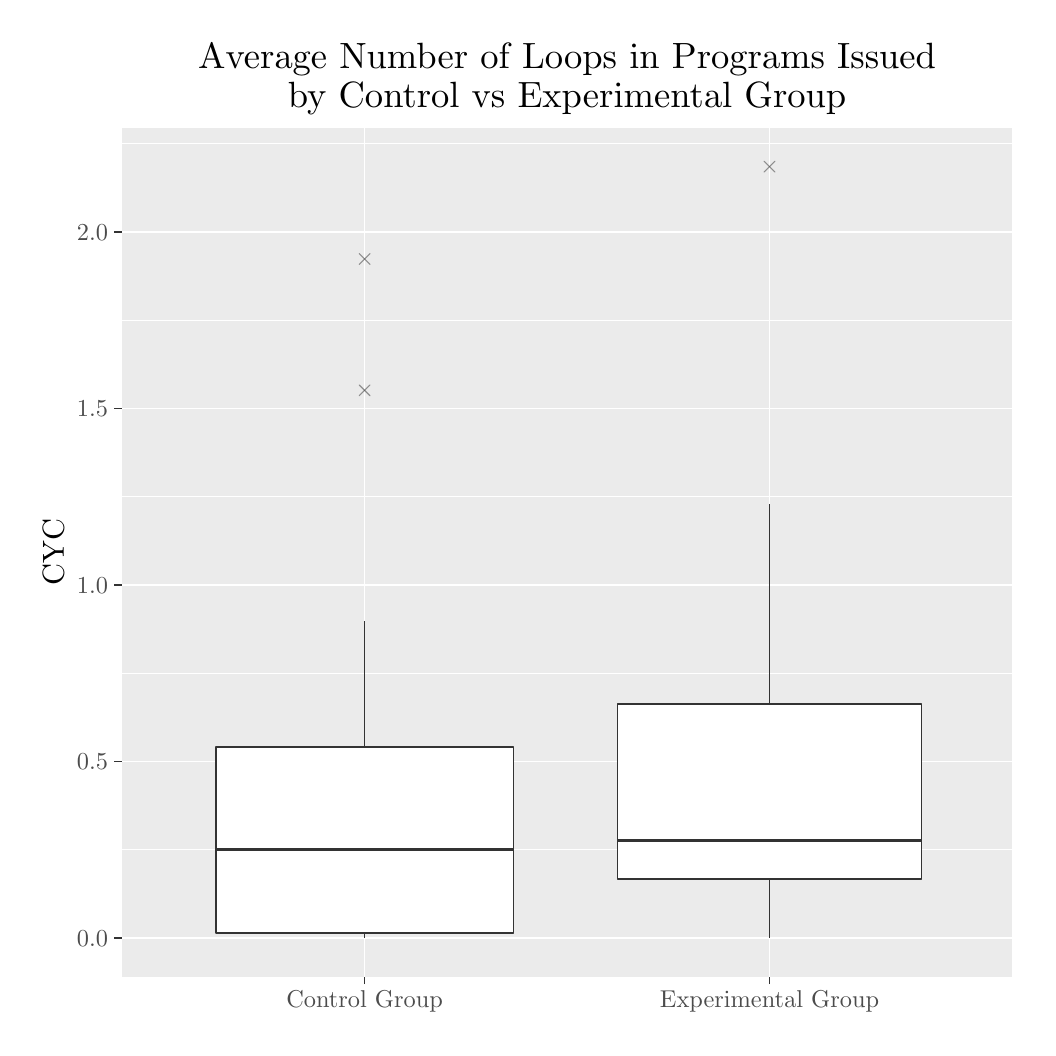
\begin{tikzpicture}[x=1pt,y=1pt]
\definecolor{fillColor}{RGB}{255,255,255}
\path[use as bounding box,fill=fillColor,fill opacity=0.00] (0,0) rectangle (361.35,361.35);
\begin{scope}
\path[clip] (  0.00,  0.00) rectangle (361.35,361.35);
\definecolor{drawColor}{RGB}{255,255,255}
\definecolor{fillColor}{RGB}{255,255,255}

\path[draw=drawColor,line width= 0.6pt,line join=round,line cap=round,fill=fillColor] (  0.00,  0.00) rectangle (361.35,361.35);
\end{scope}
\begin{scope}
\path[clip] ( 33.96, 18.45) rectangle (355.85,325.06);
\definecolor{fillColor}{gray}{0.92}

\path[fill=fillColor] ( 33.96, 18.45) rectangle (355.85,325.06);
\definecolor{drawColor}{RGB}{255,255,255}

\path[draw=drawColor,line width= 0.3pt,line join=round] ( 33.96, 64.28) --
	(355.85, 64.28);

\path[draw=drawColor,line width= 0.3pt,line join=round] ( 33.96,128.05) --
	(355.85,128.05);

\path[draw=drawColor,line width= 0.3pt,line join=round] ( 33.96,191.82) --
	(355.85,191.82);

\path[draw=drawColor,line width= 0.3pt,line join=round] ( 33.96,255.59) --
	(355.85,255.59);

\path[draw=drawColor,line width= 0.3pt,line join=round] ( 33.96,319.36) --
	(355.85,319.36);

\path[draw=drawColor,line width= 0.6pt,line join=round] ( 33.96, 32.39) --
	(355.85, 32.39);

\path[draw=drawColor,line width= 0.6pt,line join=round] ( 33.96, 96.16) --
	(355.85, 96.16);

\path[draw=drawColor,line width= 0.6pt,line join=round] ( 33.96,159.93) --
	(355.85,159.93);

\path[draw=drawColor,line width= 0.6pt,line join=round] ( 33.96,223.71) --
	(355.85,223.71);

\path[draw=drawColor,line width= 0.6pt,line join=round] ( 33.96,287.48) --
	(355.85,287.48);

\path[draw=drawColor,line width= 0.6pt,line join=round] (121.75, 18.45) --
	(121.75,325.06);

\path[draw=drawColor,line width= 0.6pt,line join=round] (268.06, 18.45) --
	(268.06,325.06);
\definecolor{drawColor}{RGB}{51,51,51}

\path[draw=drawColor,draw opacity=0.50,line width= 0.4pt,line join=round,line cap=round] (266.10,309.16) -- (270.02,313.08);

\path[draw=drawColor,draw opacity=0.50,line width= 0.4pt,line join=round,line cap=round] (266.10,313.08) -- (270.02,309.16);
\definecolor{drawColor}{gray}{0.20}

\path[draw=drawColor,line width= 0.6pt,line join=round] (268.06,117.05) -- (268.06,189.30);

\path[draw=drawColor,line width= 0.6pt,line join=round] (268.06, 53.68) -- (268.06, 32.39);
\definecolor{fillColor}{RGB}{255,255,255}

\path[draw=drawColor,line width= 0.6pt,line join=round,line cap=round,fill=fillColor] (213.19,117.05) --
	(213.19, 53.68) --
	(322.93, 53.68) --
	(322.93,117.05) --
	(213.19,117.05) --
	cycle;

\path[draw=drawColor,line width= 1.1pt,line join=round] (213.19, 67.75) -- (322.93, 67.75);
\definecolor{drawColor}{RGB}{51,51,51}

\path[draw=drawColor,draw opacity=0.50,line width= 0.4pt,line join=round,line cap=round] (119.79,275.79) -- (123.71,279.71);

\path[draw=drawColor,draw opacity=0.50,line width= 0.4pt,line join=round,line cap=round] (119.79,279.71) -- (123.71,275.79);

\path[draw=drawColor,draw opacity=0.50,line width= 0.4pt,line join=round,line cap=round] (119.79,228.34) -- (123.71,232.26);

\path[draw=drawColor,draw opacity=0.50,line width= 0.4pt,line join=round,line cap=round] (119.79,232.26) -- (123.71,228.34);
\definecolor{drawColor}{gray}{0.20}

\path[draw=drawColor,line width= 0.6pt,line join=round] (121.75,101.33) -- (121.75,146.96);

\path[draw=drawColor,line width= 0.6pt,line join=round] (121.75, 34.14) -- (121.75, 32.39);

\path[draw=drawColor,line width= 0.6pt,line join=round,line cap=round,fill=fillColor] ( 67.95,101.33) --
	( 67.95, 34.14) --
	(175.55, 34.14) --
	(175.55,101.33) --
	( 67.95,101.33) --
	cycle;

\path[draw=drawColor,line width= 1.1pt,line join=round] ( 67.95, 64.28) -- (175.55, 64.28);
\end{scope}
\begin{scope}
\path[clip] (  0.00,  0.00) rectangle (361.35,361.35);
\definecolor{drawColor}{gray}{0.30}

\node[text=drawColor,anchor=base east,inner sep=0pt, outer sep=0pt, scale=  0.88] at ( 29.01, 29.36) {0.0};

\node[text=drawColor,anchor=base east,inner sep=0pt, outer sep=0pt, scale=  0.88] at ( 29.01, 93.13) {0.5};

\node[text=drawColor,anchor=base east,inner sep=0pt, outer sep=0pt, scale=  0.88] at ( 29.01,156.90) {1.0};

\node[text=drawColor,anchor=base east,inner sep=0pt, outer sep=0pt, scale=  0.88] at ( 29.01,220.68) {1.5};

\node[text=drawColor,anchor=base east,inner sep=0pt, outer sep=0pt, scale=  0.88] at ( 29.01,284.45) {2.0};
\end{scope}
\begin{scope}
\path[clip] (  0.00,  0.00) rectangle (361.35,361.35);
\definecolor{drawColor}{gray}{0.20}

\path[draw=drawColor,line width= 0.6pt,line join=round] ( 31.21, 32.39) --
	( 33.96, 32.39);

\path[draw=drawColor,line width= 0.6pt,line join=round] ( 31.21, 96.16) --
	( 33.96, 96.16);

\path[draw=drawColor,line width= 0.6pt,line join=round] ( 31.21,159.93) --
	( 33.96,159.93);

\path[draw=drawColor,line width= 0.6pt,line join=round] ( 31.21,223.71) --
	( 33.96,223.71);

\path[draw=drawColor,line width= 0.6pt,line join=round] ( 31.21,287.48) --
	( 33.96,287.48);
\end{scope}
\begin{scope}
\path[clip] (  0.00,  0.00) rectangle (361.35,361.35);
\definecolor{drawColor}{gray}{0.20}

\path[draw=drawColor,line width= 0.6pt,line join=round] (121.75, 15.70) --
	(121.75, 18.45);

\path[draw=drawColor,line width= 0.6pt,line join=round] (268.06, 15.70) --
	(268.06, 18.45);
\end{scope}
\begin{scope}
\path[clip] (  0.00,  0.00) rectangle (361.35,361.35);
\definecolor{drawColor}{gray}{0.30}

\node[text=drawColor,anchor=base,inner sep=0pt, outer sep=0pt, scale=  0.88] at (121.75,  7.44) {Control Group};

\node[text=drawColor,anchor=base,inner sep=0pt, outer sep=0pt, scale=  0.88] at (268.06,  7.44) {Experimental Group};
\end{scope}
\begin{scope}
\path[clip] (  0.00,  0.00) rectangle (361.35,361.35);
\definecolor{drawColor}{RGB}{0,0,0}

\node[text=drawColor,rotate= 90.00,anchor=base,inner sep=0pt, outer sep=0pt, scale=  1.10] at ( 13.08,171.76) {CYC};
\end{scope}
\begin{scope}
\path[clip] (  0.00,  0.00) rectangle (361.35,361.35);
\definecolor{drawColor}{RGB}{0,0,0}

\node[text=drawColor,anchor=base,inner sep=0pt, outer sep=0pt, scale=  1.32] at (194.91,346.76) {Average Number of Loops in Programs Issued};

\node[text=drawColor,anchor=base,inner sep=0pt, outer sep=0pt, scale=  1.32] at (194.91,332.50) {by Control vs Experimental Group};
\end{scope}
\end{tikzpicture}

  \caption{Boxplot for the average number of loops issued by each group.}\label{fig:avgl}
\end{figure}

Both SEQ and CYC were not normally distributed according to the standard Shapiro-Wilk test (\(p_{SEQ} = 0.001\) and \(p_{CYC} < 0.001\)). To verify the experimental hypothesis, the one-tailed Mann-Whitney U-test was selected, which is a robust, nonparametric test.

The experimental hypothesis (\(H_1\)) predicts a difference in \ac{CT} skills development between learners working collaboratively and learners working individually. The tests were not statistically significant though (\(p_{SEQ} = 0.0658\) and \(p_{CYC} = 0.4776\)), hence the null hypothesis cannot be rejected.

\section{Discussion and Post-Hoc Analysis}
Even if the results of the experiment did not confirm the experimental hypothesis, there are interesting pointers coming from the collected data that can be helpful to explore more in-depth the main research question of this thesis and offer valid suggestions for the follow-up studies.

Results of the two evaluated measures --- SEQ and CYC --- point towards opposite effects: even though the difference is narrow, it seems that individual working groups tend to produce longer sequential programs while collaborating groups use more loops. This yet not significant effect would have been expected: by leveraging on collaboration, \acp{VPL}-based tools should foster higher-level \ac{CT} skills such as loops and abstraction, since social interactions are an important factor of constructivist learning theories, as discussed in Chapter~\ref{chap:background}. Unfortunately, the study failed to measure this sought effect (if present), and the reasons might be various and worth analysing in more detail.

First, \acp{VPL} are designed to run on traditional digital systems, which are based on a \ac{GUI} interaction paradigm: they are based on artificial control devices such as mouse and keyboard, and they don't support and take advantage of collaborative situations when multiple users are collaborating with the support of the device. A recent evolution in interaction design is indeed founded on such premise: the more modern \acp{NUI} are based on more innate human interaction paradigms such as touch, vision and speech, and are known as \emph{natural} because they rely on a user being able to carry out relatively natural motions to control the application or manipulate the on-screen content, fostering and cultivating user collaboration. Designing new and engaging tools founded on the basis of \acp{NUI} could represent a shift towards new \ac{CT} support tools, which might take more advantage of collaborative and experiential learning to better cultivate such skills.

Moreover, \ac{VPL}-based environments such as Scratch and Blockly have developed highly active online communities over the past few years, providing users with existing solutions to problems, forums to get help and discuss amongst peers, and many other resources. They were designed to take advantage of online collaboration rather than offline, representing a \ac{CT} support tool more for individual working learners, rather than collaborating ones.

The tasks provided to participants were perhaps too simple to observe a significant effect between the two experimental groups. The selected tasks were indeed real-world introductory tasks, designed to get students interested in robot programming without challenging right away inexperienced ones. Perhaps the sought effect would have been more significant with different and specifically-designed activities, but it would not have been as much grounded in existing real-world practices.

Finally, the study did not take into account more common measures such as time to task, tasks completion rates, and many other subjective measures related to attitude, engagement, and reflection. Even though these are more common measures used in the literature, the study design strived to detect \ac{CT} developments rather than programming ability. Perhaps further research on non-invasive measures of \ac{CT} skills could help highlighting this effect without designing ad-hoc evaluation tasks that might not highlight real-world effects taking place.

\section{Threats to Validity}
There are several validity threats to the design of this study.

\paragraph{Internal Validity} The limited task complexity and available time prevented a full evaluation of different \ac{CT} factors that could have influenced by the different treatments. However, the study has been conducted in a real-world scenario, with the original tasks designed by the instructors to introduce \ac{CT} to students and in their usual time schedule; even though it presents a limitation regarding research power, it offered a valid assessment of current practices and real-world effects of the evaluated tools.

\paragraph{Construct Validity} The \ac{CT} assessment was reduced to just two factors, understanding of sequences and loops; these are just two concepts related to more higher level skills defined in \ac{CT}, even though they are not explicitly mentioned by all the proposed definition outline in research. Nevertheless, these concepts were taken into account to avoid instrumenting the experiment and keep it as close as possible to real-world practices; indeed, sequences and loops comprehension can correlate with abstraction and decomposition abilities, which are two of the most mentioned \ac{CT} skills found in the literature.

\paragraph{External Validity} The results of the study can be generalized only in the context of the selected scenario, although it was carried out in a real educational setting, during an actual introductory programming session without instrumenting them. In order to generalize the findings to other scenarios though, replication studies employing different \ac{VPL}-based tools are needed.

\section{Contributions}
\replaced[comment={MP6}]{The Literature Review described in section \ref{sec:rw3} has}{Parts of the work and results described in this chapter have} been previously published in~\cite{turchi2016fostering,turchi2016human}.

\section{Conclusion}
This chapter presented an investigation on existing \ac{VPL}-based tools used in education and their effects on promoting \ac{CT} skills in a collaborative learning scenario.

A common \ac{VPL}-based system --- namely OzoBlockly --- was tested in a series of real-world introductory programming sessions, where Key Stage 3 learners collaborate to program a small robot and solve some simple tasks. The evaluation compared the effects of using such a system while collaborating with other peers and working individually, in terms of the development of \ac{CT} skills. \replaced[comment={D14}]{The study results failed to demonstrate a clear benefit of learning in collaborating groups over individual working ones in terms of \ac{CT} skills development. This requires further investigation, however it could point out how existing \ac{CT} tools favour offline collaboration, but are not specifically designed to support online collaborative learning}{Contrarily to what was expected, the results of the study did not highlight a significant benefit for collaborating groups, perhaps highlighting a lack of support to online collaboration by such tools, in favour of an offline one}. Designing tools to support online collaboration to foster \ac{CT} skills is indeed important and worth investigating whether different an interaction paradigm --- such as \acp{TUI} --- could be used to make this happen.

In the next chapter, the main research question of this thesis about the effects of tangible interaction on the development of \ac{CT} skills will be investigated in a specific application domain, namely \ac{IL} environments, where learning is self-directed and takes place as people go about their daily activities.